% Incluir dentro del documento principal y cargar referencias.bib con BibLaTeX.
\section{Causas raíz}

El 2 de junio de 2019, a las 11:45 PDT, comenzó un mantenimiento en una sola ubicación física. En las regiones afectadas, los procesos del plano de control de red y su infraestructura de soporte estaban configurados para detenerse durante el mantenimiento. Varias instancias del gestor de clústeres que ejecutaban esos procesos podían quedar incluidas en ese tipo de mantenimiento. Un error en la automatización permitió detener varios clústeres independientes a la vez, incluso en ubicaciones físicas distintas. La red siguió funcionando unos minutos hasta que se retiraron rutas BGP entre los sitios afectados y cayó la capacidad de la red \cite{googlecloud19009}. Desde fuera de Google, ThousandEyes observó pérdida de paquetes en el borde de la red en las rutas que monitoreó \cite[fig.~4]{medina2019googlecloud}.

\begin{figure}[htbp]
  \centering
  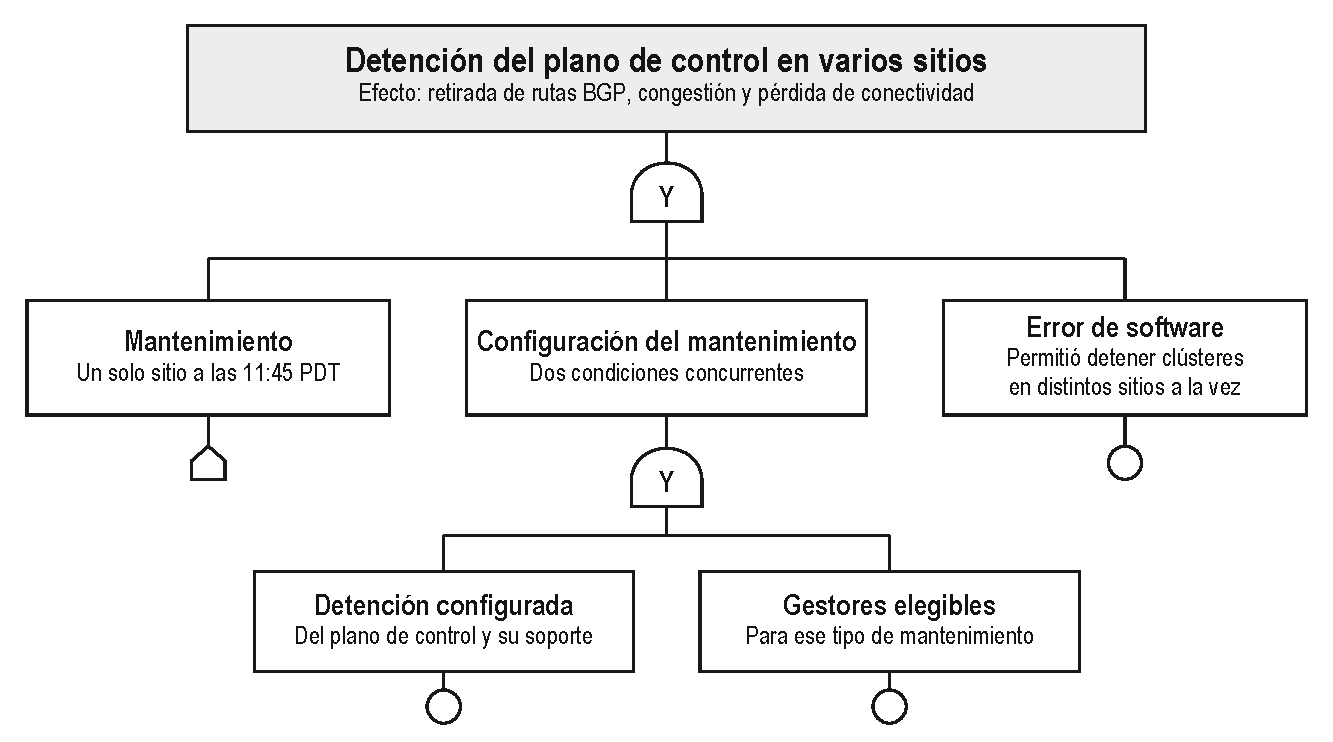
\includegraphics[width=0.88\linewidth]{diagrama-causas.pdf}
  \caption{Árbol de fallos del incidente de red. Elaborado a partir del informe de Google Cloud \cite{googlecloud19009}.}
  \label{fig:causas-google-cloud}
\end{figure}
